\documentclass[PMI,VKR]{HSEUniversity}
% Возможные опции: KR или VKR; PI или BI

\title{Dynamic Topic Modeling for Voice Dialogues}
\author{Miakov Timofey Ilich}
\supervisor{Professor NRU HSE - Nizhniy Novgorodw}{L.V. Savchenko }
\Year{2024}
\Abstract{

}

\bibliography{library.bib}

\begin{document}
\maketitle

\chapter{Introduction}

\section{Relevance of the topic}

\section{Research Objectives}
The objectives of the thesis work are:
\begin{enumerate}
    \item A review of existing approaches to dynamic text and dialogue topic modelling
    \item The definition of the main stages for DTM for audio dialogues
    \item The identification of suitable training data sets and their collection
    \item An exploration of the possibilities of using large language models for some stages and the selection of models suitable for training in limited resources
    \item The development of the architecture of all stages and their interconnections
    \item The identification of key indicators to assess the quality of each stage is also required
    \item Visual analysis of the pipeline operation on pre-selected audio data
\end{enumerate}


\chapter{Literature review}

\section{Transformer architecture}

Prior to 2017 (the publication of the original Transformer article), the main approach to working with sequences was to use Recurrent Neural Networks (RNN). However, this approach has several well-known drawbacks:

First, RNN hold all information about the sequence in a hidden state that is updated with each step. 
If the model needs to "remember" something that happened hundreds of steps ago, that information must be stored in a hidden state and not replaced with something new. 
Therefore, you either have to have a very large hidden state, or accept the loss of information.

Second, training recurrent networks is difficult to parallelize: to get the hidden state of the RNN layer for step $i$, you have to compute the state for step $i - 1$.

Both problems make it difficult to apply RNN to really long sequences: even if you wait until the end of training, your model will somehow lose information about what was at the beginning of the text. 
It is necessary to have method to "read" the sequence so that at any point in time it is possible to refer to an arbitrary point in the past in constant time and without loss of information. 
This is the self-attention mechanism underlying Transformer, introduced in "Attention is all you need" paper.

\subsection{Self-attention}

Self-attention represents a key component of the model in which tokens' information interact with each other.
At each stage of the encoder, tokens exchange information with one another, gather contextual data, and refine their previous representations (Figure 2.3). 

For each input token trainable projections $W_Q$, $W_K$, $W_V$ obtained three representations interpreted by humans as a query ($q_i$), a key ($k_i$), and a value ($v_i$).
\begin{itemize}
    \item $q_i$ - query for other tokens about the information;
    \item $k_i$ - keys that will be used to extract information about the token;
    \item $v_i$ - values of information;
\end{itemize}

Next are the attention weights that will be applied to the values from which the important information will be extracted:
\begin{center}
    $Weights_{i} = softmax(\frac{q_i \cdot k_{1}^T}{C}, \frac{q_i \cdot k_{2}^T}{C}, \dots)$,
\end{center}

where $C$ is some normalization constant, $\sqrt[]{d}$ of the dimension of keys and values was taken as a normalization constant. 

The output of the self-attention layer is a weighted sum of values with coefficients in the form of attention weights. In vectorized form, you can write:

\begin{center}
    $Attention(q, k, v) = softmax(\frac{Q \cdot K^T}{\sqrt{d_k}}) \cdot V $
\end{center}

The figure below shows the complete algorithm for the interaction of Q, K, V in the self-attention mechanism.

\begin{figure}[h]
    \centering
    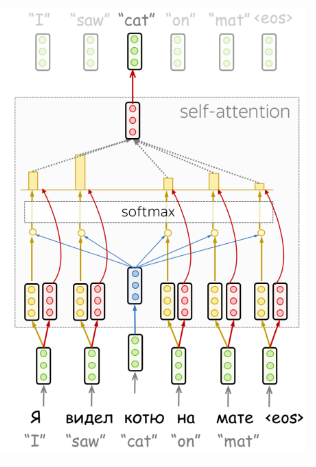
\includegraphics[scale=1]{img/query-key-value.png}
    \caption{Query, Key, Value in Self-Attention mechanism}
\end{figure}

In the decodert part the structure of the attention mechanism is different. 
They use Masked self-attention. In the form of attention described above, each token will "look" at the entire sequence, which is undesirable for the decoder. 
Indeed, in the generation stage, we will generate one token per step, and access to subsequent steps in the training stage will lead to information leakage in the decoder and poor model quality. 
To avoid this problem, you need to apply an autoregressive mask when training attention, by manually adjusting the
weights for future tokens before softmax, so that their probabilities become zero after softmax. As you can see in the image below (source), this mask has a lower triangular appearance.

\subsection{Multi-head attention}

One set of $Q, K, V$ can reflect only one type of dependency between tokens, and matrices extract only a limited amount of information from input representations. 
To compensate for this suboptimality, the authors of the architecture proposed an approach with multiple "heads" of attention (multi-head attention): 
in fact, instead of one layer of attention, we use several parallel ones with different weights, and then aggregate the results. The figure below shows what multi-head attention looks like:

\begin{figure}[h]
    \centering
    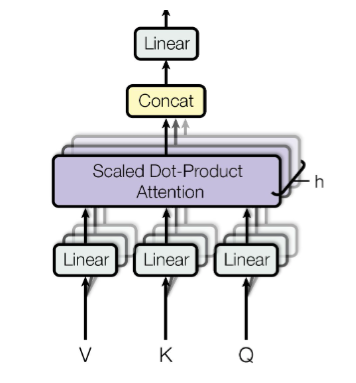
\includegraphics[scale=0.7]{img/multi-head.png}
    \caption{Query, Key, Value in Self-Attention mechanism}
\end{figure}

\subsection{Feed forward and Add \& Norm}

In addition to the attention blocks, the Transformer also contains feed-forward layers consisting of a linear layer and a ReLU activation function.
The FFN layer can be expressed as follows: \\
$FFN(x) = act(xW_{1} + b_{1}) \dot W_{2} + b_{2}$,

Intermediate activations in FFN are different: it all started with the well-known ReLU, but at some point the community switched to GELU (Gaussian Error Linear Unit) with a formula $x\Phi(x)$, where $\Phi$ - is the distribution function of a standard normal random variable
\\

The second important layer is LayerNorm, which independently normalizes the vector representation of each sequence in the batch. 
The vector representation of each token is normalized in the Transformer. In addition, LayerNorm has trainable parameters, $scale$ and $bias$, which are used after normalization to scale the output of the layer.

\begin{figure}[h]
    \centering
    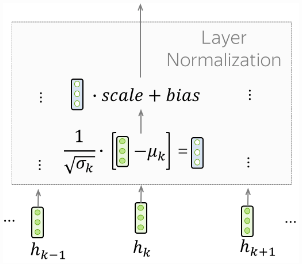
\includegraphics[scale=1]{img/layer_norm.png}
    \caption{LayerNorm слой}
\end{figure}

In Figure 2.8, note that $\mu_{k}$ and $\sigma_{k}$ are evaluated for each sequence, unlike $scale$ and $bias$, which are layer parameters.

\subsection{Positional encoding}

Since the model does not know the order of the input tokens, because all tokens are processed simultaneously, therefore we must explicitly show the model the position of the tokens. 
To do this, we have two sets of attachments: for the tokens themselves and for their positions. 
Then the input representation of the token is the sum of the two attachments.
Positional encodings can be trained, but the authors of the original article found that the presence of corrected attachments does not degrade the quality of the model. The final formula for positional embeddings looks like this:

\begin{center}
    $PE_{pos,2i} = \sin(pos/10000^{2i/d_{model}})$, \\
    $PE_{pos,2i+1} = \cos(pos/10000^{2i/d_{model}})$, \\
\end{center}
where $pos$ is a position and $i$ is a vector dimension. Each measure of position encoding corresponds to a sine wave, and the wavelengths form a geometric progression from $2\pi$ to 10,000$\cdot 2\pi$.

\begin{figure}[h]
    \centering
    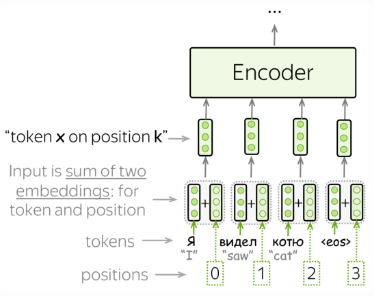
\includegraphics[scale=1]{img/pos_encoding.png}
    \caption{Positional encoding}
\end{figure}

A newer version of positional encoding is rotary embeddings.
Rotary Position Embedding, or RoPE, is a type of position embedding that encodes absolute position information with a rotation matrix and naturally incorporates explicit relative position dependency into the self-attention formulation. 
In particular, RoPE has valuable properties such as the flexibility to be extended to arbitrary sequence lengths, decaying inter-token dependency with increasing relative distances, and the ability to augment linear self-attention with relative position encoding. 

\begin{figure}[h]
    \centering
    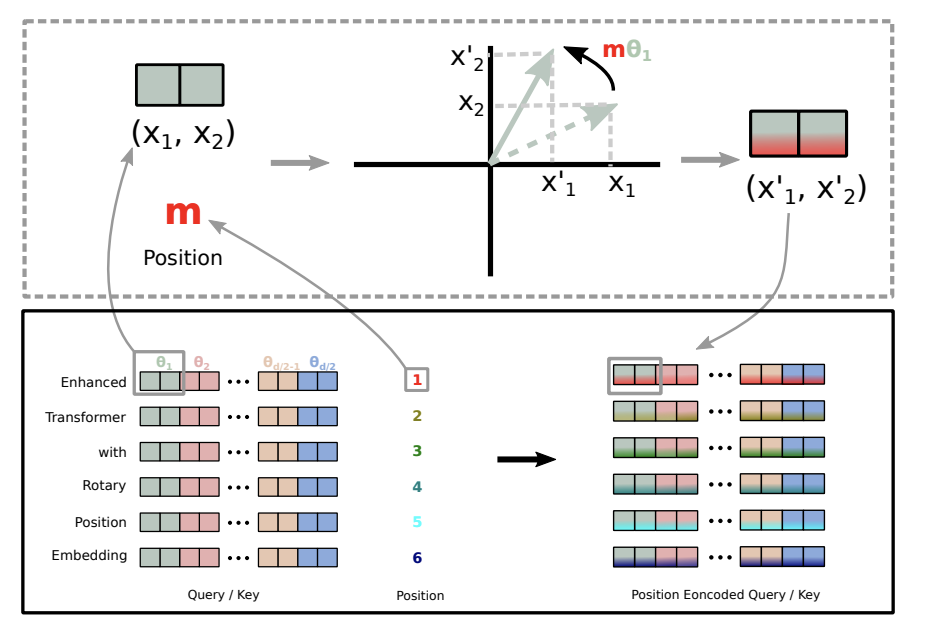
\includegraphics[scale=0.7]{img/rotary_embs.png}
    \caption{Rotary embeddings}
\end{figure}

\section{BERT}

The BERT is a language model based on the transformer architecture, that was first introduced in the article BERT: Pre-training of Deep Bidirectional Transformers for Language Understanding\cite{bert:2018}.  
From an architectural point of view, BERT consists of 12 encoder blocks, including a Self-Attention mechanism, Normalization and Feed-forward layers.

\begin{figure}[h]
    \centering
    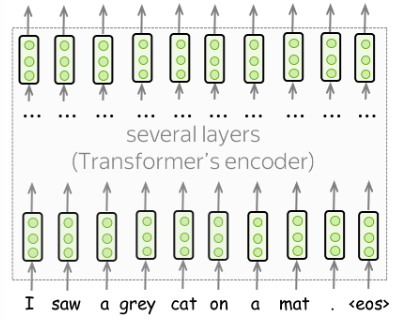
\includegraphics[scale=0.8]{img/bert.png}
    \caption{BERT architecture}
\end{figure}


\subsection[short]{Training tasks}
BERT has two pretrain objective described in article: \\
The first objective of the training process is the masked language modelling (MLM). 
During the training phase of MLM, the following occurs:

\begin{itemize}
    \item A number of tokens are selected with a probability of 15\% for each token.
    \item The selected tokens are replaced by [MASK] with a probability of 80\%, a random token with a probability of 15\% and remain unchanged with a probability of 10\%.
    \item The model must predict the original token.
\end{itemize}

Secondly, Next Sentence Prediction (NSP) task is a binary classification task. 
In order to understand relationship between two sentences, BERT training process also uses next sentence prediction.
During training the model gets as input pairs of sentences and it learns to predict if the second sentence is the next sentence in the original text as well. 
The training dataset presented in the original paper states that when trained, 50\% of the examples contain related sentences extracted from the training texts, while the remaining 50\% contain a random pair of sentences.


\section{Large Language models}


\subsection{LLaMA}


\subsection{Mistral}



The pipeline of dynamic thematic modelling of audio dialogues, which will be considered in this paper, is divided into several main stages. 
These include audio-to-text, dialogue segmentation, topic extraction, and topic evolution. 
The approaches and algorithms used in these stages will be described in detail from a theoretical point of view.


\section{Automatic Speech Recognition Stage}


\section{Dialogue Segmentation Stage}

The dialogue segmentation stage represents the initial stage for textual type of data. 
The result is a set of utterance indices that indicate the beginning of a thematically related group. 

In accordance with the majority of previous studies, we have utilise the best open-source solution based on the presented in papers metrics. 
It is algorithm from Improving Unsupervised Dialogue Topic Segmentation with Utterance-Pair Coherence Scoring by Linzi Xing and Giuseppe Carenini (2020)
Let us now examine the algorithm in greater detail. 

In terms of our approach to topic segmentation, authors utilise Next Sentence Prediction (NSP) BERT as the encoder, due to the similarity of these two tasks. 
Both tasks take a pair of sentences/utterances as input, with the objective of predicting the appropriate next sentence, which should be topically related. 

In more detail, the positive instances $(s_{i}, s_{t+i})$ and negative instances $(s_{i}, s_{t-i})$ are fed into the model in the form of the following sequence: 
\begin{center}
    $[CLS] s_{i} [SEP] s_{t+/-i} [SEP]$,
\end{center}
where the symbols $[CLS]$ and $[SEP]$ represent special tokens in BERT. 

Here, the contextualised representation of $[CLS]$ is employed as the topic-aware embedding to predict the degree of matching between the two input utterances in terms of topic. 
The topic coherence scores are estimated by passing the $[CLS]$ representation through another MLP.


\subsection{Depth Scores calculation}

The input of stage is a set of utterances $\{u1, u2, ..., uk\}$. 
Subsequently, an utterance-pair coherence scoring model is applied to $k - 1$ consecutive pairs, resulting in a sequence of coherence scores $\{c1, c2, ..., ck-1\}$. 
The value of $c_i \in [0, 1]$ indicates the topical relatedness of the two utterances in the $i_th$ pair. 
The algorithm utilises coherence scores as a foundation idea, yet enhances them through the sequence of "depth scores". $\{dp1, dp2, ..., dpk-1\}$ is calculated to measure the sharpness of a valley. 
This is achieved by examining the highest coherence scores $h_l(i)$ and $h_r(i)$ on either side of interval $i$.

The depth score for interval $i$, $dp_i$, is calculated as follows: 
\begin{center}
    $D_{pi} = \frac{h_{l}(i) + h_{r}(i) - 2 \cdot c_{i}}{2}$. 
\end{center}

A higher depth score indicates a lower topical relatedness between the pair of utterances. 
The threshold $\tau$, which is used to identify segment boundaries, is computed from the mean $\mu$ and standard deviation $\sigma$ of depth scores: $\tau = \mu - \frac{\sigma}{2}$. 
A pair of utterances with a depth score exceeding $\tau$ will be selected to have a segment boundary between them. 


\section{Topic Extraction Stage}


\subsection{LLM for topic extraction}


\section{Topic Evolution over time}






\newpage
\chapter{Experiments}

Основной задачей в работе будет классификация видео на наличие юмора с использованием разных моделей для разных модальностей.
Для работы с разными модальностями будут использованы 3 модели, которые были описаны в теоретической части:
\begin{itemize}
    \item Wave2Vec - извлечение аудио признаков,
    \item BERT - извлечение текстовых признаков,
    \item TimeSFormer - извлечение признаков из видео фрагментов,
\end{itemize}

Сначала модели попробуют предсказать классы в своих модальностях, после чего их предсказания будут обработаны вместе для улучшения результатов.

\section{Классификация по одной модальности}

Для извлечения признаков, как уже было описано, будут использоваться 3 различные модели. В силу ограниченных вычислительных мощностей, будут взяты предобученные модели с \href{https://huggingface.co/}{Hugging Face} и дообучены на наших данных.

Так как у нас ровное кол-во наблюдений положительного и отрицательного классов, делим выборку 70\% на дообучение и 30\% валидацию с одинаковым кол-вом примеров разных классов в обеих подвыборках.

Для каждой модели начала посчитаем качество модели по 3 метрикам: Accuracy (из-за отличной балансировки, можем использовать обычную accuracy), Precision, Recall.

\begin{itemize}
    \item Для работы с текстом будем использовать RoBERTa из библиотеки моделей HuggingFace: \href{https://huggingface.co/roberta-base}{roberta-base}.
    \item Для работы с аудио будем использовать Wave2vec2 из библиотеки моделей HuggingFace: \href{https://huggingface.co/facebook/wav2vec2-base}{wav2vec2-base}.
    \item Для работы с видео будем использовать Wave2vec2 из библиотеки моделей HuggingFace: \href{https://huggingface.co/facebook/timesformer-base-finetuned-k400}{timesformer-base}.
\end{itemize}

С помощью предлагаемых Hugging Face интрументов, сделаем дообучение моделей под нашу задачу. \\

\subsection{Результаты}

\textbf{Далее в таблицах с результатами модальности будут называться в сокращенном виде: Текст - Т, Аудио - А, Видео - В.} \\

Результаты классификации по одной модальности: \\

\begin{center}
    \begin{tabular}{ |c||c|c|c|}
        \hline
        \multicolumn{4}{|c|}{Классификация по тексту} \\
        \hline
        Модальность & Accuracy & Precision & Recall   \\
        \hline
        Т           & 0.71377  & 0.70563   & 0.75064  \\
        В           & 0.47836  & 0.50600   & 0.59729  \\
        А           & 0.50885  & 0.57865   & 0.78420  \\
        \hline
    \end{tabular} \\
\end{center}



TimeSFormer показывает достаточно низкие значени метрик, относительно других моделей. Такие результаты связаны со спецификой задачи, моедль не фоксируется только на человеке, но на всем видеофрагменте. Возможным решением станет использование других моделей или инструментов, которые будут обрабатывать именно человека на видео.

Wave2vec показывает хороший recall (т.е модель хорошо угадывает, класс с юмором), но accuracy все еще плохой.

По результатам можем сделать вывод, что самым подходящей для детекции юмора оказалась текстовая модальност, с которой работала RoBERTa. Действительно по тексту легче всего понять, есть ли шутка, потому что не надо обрабатывать много второстепенной информации, как в видео, и "поведение"\ голоса разных людей во время шутки, как на аудио.

\section{Классификация видео с использованием нескольких модальностей}

Теперь попробуем собирать вместе голосование моделей в разных модальностях, сначала будем брать все комбинации 2 модальностей, а потом возьмем 3 модальности.

Подсчет результатов будем производить двумя разными сопобами:
\begin{itemize}
    \item Посчитать среднюю вероятность
    \item Выбирать голосованием, каждой модели за класс
\end{itemize} \\

\subsection{Результаты}

Результаты экспериментов с подсчетом средней вероятности: \\

\begin{center}
    \begin{tabular}{ |c||c|c|c| }
        \hline
        Модальности & Accuracy & Precision & Recall  \\
        \hline
        А + В       & 0.49737  & 0.50512   & 0.60373 \\
        А + Т       & 0.71377  & 0.70488   & 0.75257 \\
        В + Т       & 0.63573  & 0.63569   & 0.66559 \\
        А + В + Т   & 0.63081  & 0.62862   & 0.67074 \\
        \hline
    \end{tabular}
\end{center} \\

В голосованиях в парах и тройке результаты лучше, чем у А и В по одиночке.
А + Т слегка улучшает результат RoBERTa в одиночку, а в остальных парах и тройке, результаты улучшаются, но не достигают RoBERTa.


При спорных ситуациях в голосованием по классам, решающий голос за модальностями с лучшим результатом в прошлой частью (т.е. TimeSFormer имеет самый слабый голос, затем Wave2Vec и самый сильный голос у RoBERTa).

Результаты экспериментов с голосованием по классам: \\

\begin{center}
    \begin{tabular}{ |c||c|c|c|}
        \hline
        Модальности & Accuracy & Precision & Recall  \\
        \hline
        А + В       & 0.49737  & 0.50512   & 0.60373 \\
        А + Т       & 0.71377  & 0.70563   & 0.75064 \\
        В + Т       & 0.71377  & 0.70563   & 0.75064 \\
        А + В + Т   & 0.50885  & 0.50885   & 1.0     \\
        \hline
    \end{tabular}
\end{center} \\

Здесь можно заметить, т.к. текст имеет решщающий голос, то в парах с текстом результаты одинаковые.
В А + В + Т интересно заметить, что recall равен 1.0. Тоесть наша "тройка"\ относит все сэйплы к одному классу.


\chapter{Заключение}

В ходе проделанной работы были прочитаны статьи в разделе нейронных сетей, изучен механизм внимания и архитектура Трансформер с теоретической точки зрения. Также изучены модели, в основе которых лежит Трансформер: RoBerta, используемая для работы с текстовой модальностью, Wave2vec2, используемая для работы с звуковой модальностью, и TimeSFromer, используемая для работы с визуальной модальностью.

Далее были проведены эксперименты  на датасете UrFunnny с каждой из моделей. Изучив результаты можно увидеть, что RoBERTa показыает самые хорошие результаты. Предположения, почему получились такие результаты было сделано в пунке 3.1.1 под таблицей с результатами.

Что касается совмещения результатов моделей (голосование по вероятностям и финальным лэйблам), аудио и текст вместе улучшают результат RoBERTa в одиночку.

Для работы с моделями, обучение и инференс, был изучен фрэймворк HuggingFace, имеющий большую популярность в сфере глубокого обучения. Кроме того были использованы язык программирования Python, PyTorch - бекэнд для нейронных сетей, а также вспомогательные библиотеки librosa (работа со звуком) и Numpy.

Следующим шагом в исследовании детекции юмора может стать объединением моделей в одну, на примере CLIP от openAI или улучшение моделей в аудио и видео модальностях.




\putbibliography %Вместо этой команды будет вставлена библиография

\end{document}